\documentclass[12pt]{article}
\usepackage[margin=3cm]{geometry}
\usepackage[utf8]{inputenc}
\usepackage[T1]{fontenc}
\usepackage[german]{babel}
\usepackage{array}
\usepackage{amsmath}
\usepackage{graphicx}
\usepackage{rotating}
\usepackage{float}
\usepackage{enumitem}
\usepackage[export]{adjustbox}
\usepackage[dvipsnames]{xcolor}
\usepackage{listings}
\usepackage{fancyhdr}
\usepackage{ragged2e}

% Style für inkludierten Code definieren
\lstdefinestyle{mystyle}{
	backgroundcolor=\color{white},
	commentstyle=\color{gray},
	keywordstyle=\color{magenta},
	numberstyle=\footnotesize\color{gray},
	stringstyle=\color{purple},
	basicstyle=\ttfamily\footnotesize,
	breakatwhitespace=false,
	breaklines=true,
	columns=fullflexible,
	postbreak=\raisebox{0ex}[0ex][0ex]{$\hookrightarrow$\space},
	captionpos=b,
	keepspaces=true,
	numbers=left,
	numbersep=5pt,
	showspaces=false,
	showstringspaces=false,
	showtabs=false,
	tabsize=2
}
\lstset{style=mystyle}

% JSON styling
\definecolor{delim}{RGB}{20,105,176}
\definecolor{numb}{RGB}{106, 109, 32}
\lstdefinelanguage{json}{
    morestring=[b]",
    stringstyle=\color{purple},
    literate=
     *{0}{{{\color{numb}0}}}{1}
      {1}{{{\color{numb}1}}}{1}
      {2}{{{\color{numb}2}}}{1}
      {3}{{{\color{numb}3}}}{1}
      {4}{{{\color{numb}4}}}{1}
      {5}{{{\color{numb}5}}}{1}
      {6}{{{\color{numb}6}}}{1}
      {7}{{{\color{numb}7}}}{1}
      {8}{{{\color{numb}8}}}{1}
      {9}{{{\color{numb}9}}}{1}
      {\{}{{{\color{delim}{\{}}}}{1}
      {\}}{{{\color{delim}{\}}}}}{1}
      {[}{{{\color{delim}{[}}}}{1}
      {]}{{{\color{delim}{]}}}}{1},
}

% header configuration
\renewcommand{\headrulewidth}{0pt}

\begin{document}
	% Für fancy headers
	\pagestyle{fancy}
	\fancyhf{}
	%\setlength{\parindent}{0pt}
	
	% Keine Seitennummern von Titelblatt bis Inhalt
	\pagenumbering{gobble}
	
	% Titelblatt
	\begin{titlepage}
		\centering
		\Huge
		\begin{figure}[H]
			
\includegraphics[width=1\textwidth, center]{img/HTL_Logo.png}
		\end{figure}
		\textbf{Diplomarbeit} \\
		\vspace{5mm}
		\huge
		SwarmBots \\ 
		\vspace{5mm} 
		Schuljahr 2024/25 \\
		\vspace{2cm}
		\Large
		\begin{tabular}{r @{: } >{\bfseries} l r}
			\vspace{3mm}
			Betreuer & Dipl.-Ing Erich Erker\\
			Gruppenmitglieder & Arthur Burjak & | 5AHEL\\
			& Leander Gastgeber & | 5AHEL\\
			& Jones Soliman & | 5AHEL\\
			& Mihael Stojkovic & | 5AHEL 
	\end{tabular}
	\end{titlepage}
	\newpage
	\centering
	\LARGE
	\textbf{Erklärung über die eigenständige Verfassung der Diplomarbeit}

	\justify 
	\Large
	Wir, die Herren Arthur Burjak, Leander Gastgeber, Jones Soliman und Mihael Stojkovic, Schüler
	der Klasse 5AHEL der Höheren Technischen Bundeslehranstalt Wien 10, erklären hiermit an
	Eides statt, dass wir die vorliegende Diplomarbeit selbständig und ohne fremde Hilfe verfasst
	haben, einschließlich auch andere als die angegebenen Quellen und Hilfsmittel nicht benutzt
	und die benutzten Quellen, wörtlich und inhaltlich entnommenen Stellen, als solche
	erkenntlich in der Diplomarbeit gekennzeichnet haben
	\\
	\vspace{5mm}
	\\
	Wien, am 11.04.2025
	\vspace{8mm} \\

	\begin{tabular}{l c r}
		\vspace{3mm}
		Verfasser: \\
		Arthur Burjak & | 5AHEL & U:\rule{5cm}{0.4pt}	\\
		Leander Gastgeber & | 5AHEL & U:\rule{5cm}{0.4pt} 	\\
		Jones Soliman & | 5AHEL & U:\rule{5cm}{0.4pt}	\\
		Mihael Stojkovic & | 5AHEL & U:\rule{5cm}{0.4pt}
	\end{tabular}
	
	\normalsize
	\newpage
	% Inhaltsverzeichnis wird hier generiert
	\tableofcontents
	\newpage
	
	\pagenumbering{arabic}
	\fancyhead[L]{5AHEL 2024/25}
	\fancyhead[R]{SwarmBots}
	\fancyfoot[C]{\thepage/\pageref{_LASTPAGE}}

	%% Hier beginnt der tatsächliche Inhalt
	% TODO: Kapitel in mehrere Dateien aufteilen?
	\section{Zusammenfassung}
	Ziel dieser Diplomarbeit ist es, drei Roboter zu entwickeln,
	welche kooperativ die Umgebung erkunden können.
	%
	Hierbei ist ein Roboter (``Guide'') mit einem LiDAR-Sensor ausgestattet,
	welcher Entfernungsmessungen durchführt.
	%
	Die anderen beiden Roboter (getauft ``Tamerlan'' und ``Bambi'')
	sollen komplett ``blind'' sein.
	%
	Koordiniert wird das ganze über einen zentralen Server,
	welcher die gesammelten Daten zusätzlich über ein Webinterface darstellt.
	%
	Als zusätzliche Aufgabe sollen sich die Roboter auf nur einer Achse balancieren,
	da wir Kits für balancierende Roboter verwenden,
	welche wir für unsere Zwecke modifiziert haben.
	Die Software basiert auf den Robotern,
	die wir letztes Jahr im Zuge der Projektwoche als Vorbereitung auf die Diplomarbeit gebaut haben.
	\subsection{Abstract (English)}
	Goal of this diploma thesis is to develop three robots which
	can explore the environment cooperatively.
	%
    One robot (``Guide'') is equipped with a LiDAR sensor,
    which carries out distance measurements.
	%
	The other two robots (named ``Tamerlan'' and ``Bambi'')
    are to be completely ``blind''.
	%
	The diploma thesis is coordinated via a central server,
    which also displays the collected data via a web interface.
	%
	As an additional task, the robots should balance themselves on only one axis,
    as we use kits for balancing robots,
    which we have modified for our purposes.
    The software is based on the robots
    that we built last year during the project week in preparation for the diploma thesis.
	\section{Projektstart}
	\section{Prototyp}
	Im Zuge der Projektwoche im Schuljahr 2023/24 haben wir bereits begonnen,
	einen ersten Prototypen unseres SwarmBots-Systems zu bauen.
	%
	Dieser Prototyp bestand aus nur zwei Robotern,
	welche auf Basis eines fertigen Fahrgestells zu sehr wackligen Gefährten wurden.
	%
	Sehr viel Autonomie hatten die früheren Roboter auch noch nicht,
	der LiDAR war noch nicht funktionstüchtig,
	stattdessen wurden die Roboter mittels Videospiel-Controller ferngesteuert.
	%
	Diese Fernsteuerung wurde aber auch schon damals über eine Websocket-Verbindung implementiert.
	%
	Außerdem wurde während der Projektwoche der Code für die ESP32-CAMs fast komplett fertiggestellt,
	diese verwenden jetzt immer noch größtenteils das gleiche Programm.
	%
	Trotz der Schwächen des damaligen Systems wurde unserem Projekt
	der erste Preis in der Kategorie ``Experten'' verliehen.
	%TODO Bilder zu Projektwoche
	\section{Erster Roboteraufbau}
	\subsection{Elegoo Tumbller Kit}
	\label{elegoo_tumbller}
	Um den Hardwareaufbau so einfach wie möglich zu gestalten,
	entschieden wir uns dafür,
	fertig entwickelte Kits online zu bestellen und dann zu modifizieren.
	%
	Die Wahl des Kits fiel letztendlich auf den ``Tumbller'' von Elegoo (Siehe Abbildung \ref{fig:elegoo_tumbller}).
	%
	Der Tumbller ist ein zweirädriger Roboter, welcher auf einer Ache balanciert.
	%
	Zur Kontrolle des unmodifizierten Kits gibt es eine Smartphone-App,
	welche die Roboter über Bluetooth fernsteuern kann.
	%TODO genaue Hardwarebeschreibung des Kits
	%
	Da wir die Roboter über WLAN steuern wollten, 
	und die Tumbller-Kits standardmäßig nur eine Bluetooth-Erweiterung eingebaut haben,
	haben wir die mitgelieferten Arduino Nano durch ESP32-Boards im Arduino Nano-Format ersetzt.
	% TODO Spannungsunterschiede Arduino Nano vs ESP
	\begin{figure}[H]
		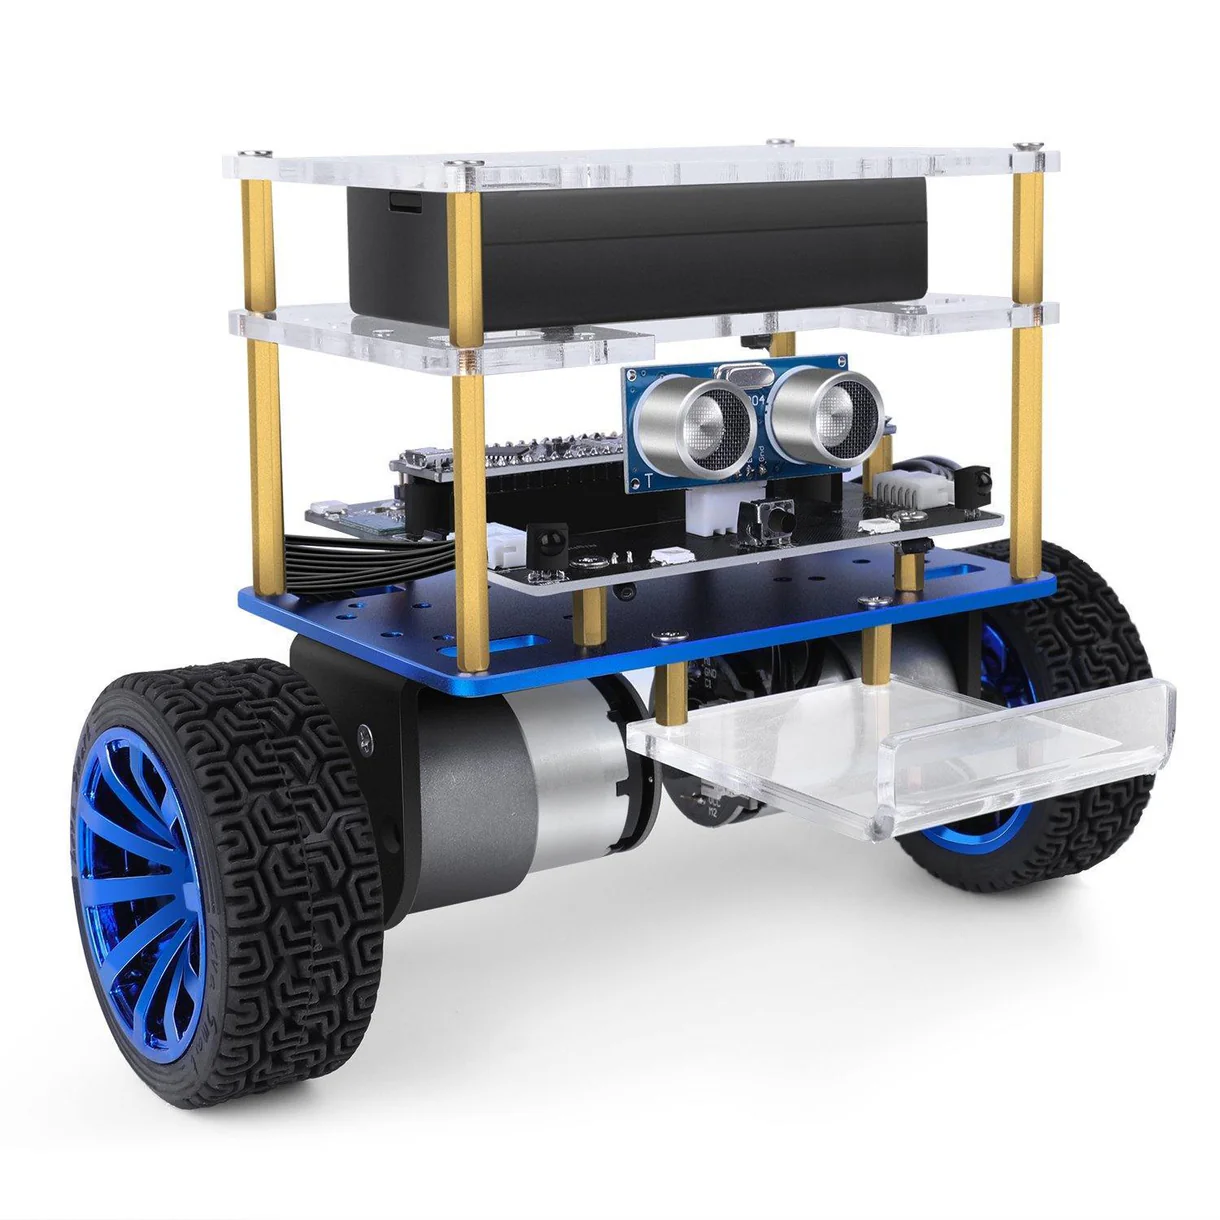
\includegraphics[width=0.7\textwidth, center]{img/elegoo_tumbller.png}
		\caption{Rendering des Elegoo Tumbller}
		\label{fig:elegoo_tumbller}
	\end{figure}
	\begin{sidewaysfigure}
		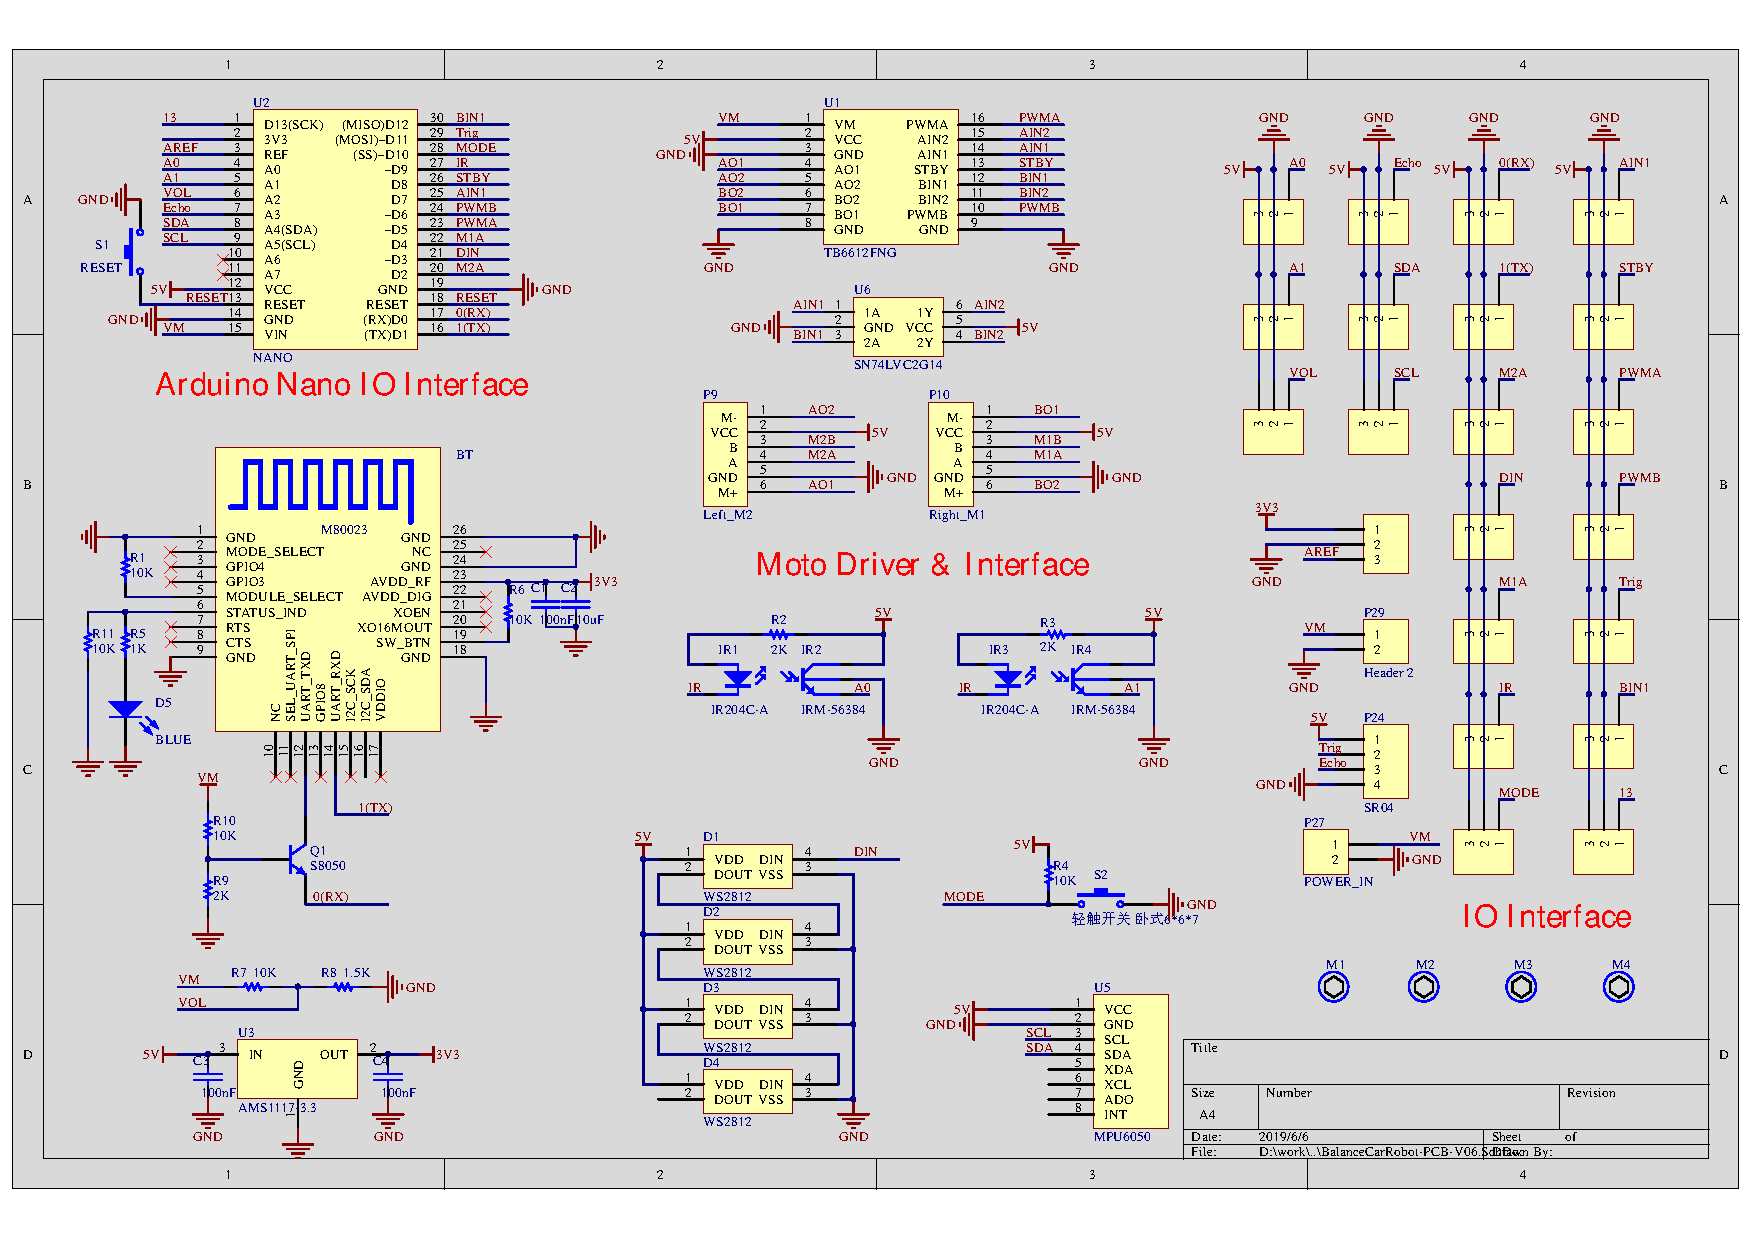
\includegraphics[width=\textwidth, center]{img/elegoo_tumbller_original_circuit.pdf}
		\caption{Originaler Schaltplan des Tumbllers (TODO: neu zeichnen)}
		\label{fig:elegoo_tumbller_original_circuit}
	\end{sidewaysfigure}

	\subsection{Guide}
	Die Aufgabe von \textit{Guide} ist es,
	mithilfe eines LiDAR-Sensors (Siehe Kapitel \ref{lidar}) die Umgebung nach Hindernissen
	und den anderen Robotern abzusuchen.
	%
	Die vom LiDAR gesammelten Abstandsdaten werden über eine TCP/IP Websocket-Verbindung
	an einen zentralen Server weitergegeben,
	welcher diese weiter verarbeitet.
	%
	Um den LiDAR-Sensor zu montieren,
	haben wir das Fahrgestell leicht modifiziert
	und die oberste Ebene (mit dem Akku) erhöht,
	um Platz für Schrauben zu schaffen.
	\subsection{Tamerlan \& Bambi}
	\section{Programmierung}
	Für die Programmierung der Mikrocontroller verwenden wir PlatformIO.
	%
	PlatformIO ist eine Alternative zur Arduino-IDE,
	welche mithilfe von Plugins in viele IDEs wie z.B. VSCode und CLion integriert werden kann.
	%
	Alternativ kann man PlatformIO auch über die Kommandozeile bedienen.
	%
	Vorteile von PlatformIO gegenüber der Arduino-IDE sind u.A. schnelleres Kompilieren,
	ordentliche Auto-Vervollständigung,
	statische Code-Analyse (Linting),
	und ein schön geregeltes System für Bibliotheken.
	%TODO eigenes (Unter-)Kapitel für PlatformIO?
	%TODO eigenes (Unter-)Kapitel für VSC&Plugins?
	%TODO eigenes (Unter-)Kapitel für Protobufs!

	\subsection{ESP32-CAM}
	Wir verwenden jeweils ein ESP32-CAM AI-Thinker Modul zur erweiterten
	Fernüberwachung der Roboter.
	%
	Dieses verbindet sich über WLAN mit dem \texttt{IoT}-Netzwerk und bietet über HTTP einen MJPEG-Videostream an.
	%
	Die drei Videostreams (einer pro Roboter) werden dann im Web-Interface
	zusätzlich zu den LiDAR-Umgebungsdaten angezeigt,
	um das räumliche Vorstellungsvermögen der Benutzer zu unterstützen.
	\begin{figure}[H]
		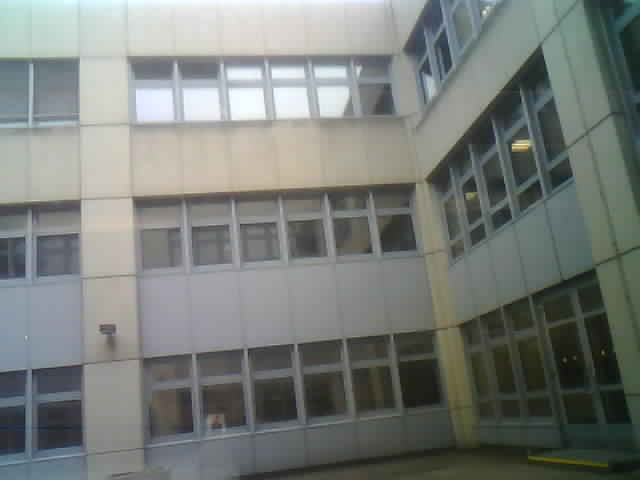
\includegraphics[width=0.7\textwidth, center]{img/cam_erstes_bild.png}
		\caption{Erstes empfangenes Bild der ESP32-CAM}
		\label{fig:cam_erstes_bild}
	\end{figure}
	\subsection{Sensoren}
	\subsubsection{LiDAR}
	\label{lidar}
	\subsubsection{Gyroskop}
	\subsubsection{Encoder}
	\section{Backend-Server}
	\subsection{Datenverwaltung}
	\subsection{Roboterpositionen}
	\section{Web-Interface}
	\subsection{LiDAR-Karte}
	\subsection{Anzeigen der Sensordaten}
	\subsection{Fernüberwachung per Kamera}
	\section{Probleme}
	\subsection{Docker}
	%TODO wording?
	Am Laptop von Herr Gastgeber war es am Beginn des Schuljahres nicht möglich,
	jegliche Geräte im Netzwerk der HTL zu erreichen.
	%
	Grund dafür war eine Software namens Docker,
	welche außerhalb dieses Projekts zur Containerisierung von anderen Anwendungen dient.
	%
	Docker war standardmäßig so konfiguriert,
	dass es containerspezifische Subnets im IPv4-Adressbereich \allowbreak\texttt{172.117.0.0/16} erstellt.
	%
	Diese Subnets hatten dann am Laptop eine höhere Priorität als das Schulnetzwerk,
	was dafür sorgte,
	dass das weltweite Internet noch erreichbar war, 
	nicht aber das lokale Schulnetzwerk.
	%
	Um Docker einen anderen IP-Adressbereich zuzuweisen,
	wurde der Docker-Daemon mithilfe der Datei \texttt{/etc/docker/daemon.json}
	wie in Listing \ref{lst:docker-address-pools} konfiguriert.
	\begin{lstlisting}[language=json,gobble=4,
		label=lst:docker-address-pools,caption=Konfiguration für den Docker-Daemon]
		{
  			"default-address-pools":
  			[
    			{"base":"10.10.0.0/16","size":24}
  			]
		}
	\end{lstlisting}

	\subsection{Modifikationen am Tumbller}
	Als wir das Projekt geplant haben,
	war die Idee,
	einfach ein fertiges Kit ein bisschen zu modifizieren,
	fast schon zu schön um wahr zu sein.
	%
	Und das war es dann auch.
	%
	Bei den Hardware-Modifikationen am Tumbller (siehe Kapitel \ref{elegoo_tumbller}) gab es zwei relativ große Probleme:

	\subsubsection{Falsche Betriebsspannungen}
	\label{problem_betriebsspannungen}
	Beim Austausch des mitgelieferten Arduino Nano mit einem ESP32 im Nano-Format haben wir einen wichtigen Faktor übersehen:
	%
	Der Arduino Nano hat eine Betriebsspannung von 5V,
	während der ESP32 mit 3.3V arbeitet.
	%
	Glücklicherweise funktionieren die meisten Komponenten des Elegoo Tumbllers auch mit 3.3V.
	%
	Die einzigen Bauteile,
	welche eine höhere Spannung benötigen,
	sind die auf der Platine angelöteten farbigen Leuchtdioden.
	%
	Um nicht das ganze Projekt von Grund auf neu aufbauen zu müssen,
	haben wir uns entschieden,
	dieses kleine optische Detail fürs Erste auszulassen.
	%
	%TODO schaltplan
	In der originalen Beschaltung (siehe Abbildung \ref{fig:elegoo_tumbller_original_circuit})
	wurde das Bluetooth-Modul mithilfe des Spannungswandlers \texttt{U3} mit 3.3V versorgt.
	%
	Diesen Spannungswandler haben wir ausgebaut und mittels einer Lötbrücke $V_{in}$ mit $V_{out}$ verbunden.
	Allerdings erwies sich das Bluetooth Modul später als problematisch (siehe Kapitel \ref{problem_bluetooth_serial}),
	weshalb die Überbrückung eigentlich nicht notwendig ist.
	\\\\
	Außerdem war es beim Guide-Roboter aufgrund des Wechsels auf 3.3V nicht mehr möglich,
	den LiDAR-Sensor direkt mit dem Spannungswandler des Mikrocontroller-Boards zu versorgen.
	%
	Deshalb haben wir für den Guide einen zusätzlichen Step-Down-Konverter eingebaut,
	welcher die Versorgungsspannung des Akkus auf 5V für den LiDAR herunterregelt.
	\subsection{Blockierte UART-Schnittstelle}
	\label{problem_bluetooth_serial}
	Als das Problem der inkompatiblen Spannungen gelöst,
	und die erste Version des Programmes zum Testen der einzelnen Komponenten geschrieben war,
	%TODO Formulierung: "großes Problem" hab ich schon vorher verwendet
	sind wir auch schon auf das nächste nennenswerte Problem gestoßen:
	%
	Das externe Bluetooth-Modul,
	was bereits auf der Platine verlötet war,
	belegt die UART-Schnittstelle des eingebauten ESP32.
	%
	Das führte dazu, dass der ESP32 nur neu programmiert werden konnte,
	wenn das ESP32-Devboard aus dem Roboter ausgebaut war.
	%
	Außerdem wurde dadurch das Debuggen mittels UART über USB unmöglich gemacht.
	\\
	Da wir die Roboter über WLAN steuern,
	und der ESP32 auch ohne externe Erweiterungen bereits sowohl über WLAN- als auch Bluetooth-Kapazitäten verfügt,
	haben wir entschlossen,
	die mitgelieferte Platine weiter zu modifizieren,
	indem wir das Bluetooth-Modul entfernen.
	%
	Außerdem haben wir den Transistor \texttt{Q1} und den Spannungsteiler,
	welcher aus \texttt{R9} und \texttt{R10} besteht entfernt,
	um sicherzustellen, das die UART-Verbindung keinesfalls beeinflusst wird
	(siehe Original-Schaltplan in Abbildung \ref{fig:elegoo_tumbller_original_circuit}).
	%TODO Bilder und Erläuterung zu Entfernen des Bluetooth Moduls

	% Abbildungs- und Tabellenverzeichnis
	\newpage
	\begin{appendix}
		\addcontentsline{toc}{section}{Abbildungsverzeichnis}
		\listoffigures
		\addcontentsline{toc}{section}{Tabellenverzeichnis}
		\listoftables
	\end{appendix}
	% Special label used for the page counter on the footer
	\label{_LASTPAGE}
\end{document}